\subsection{Case Study: Web eID}

\subsubsection{About}

Released in the Summer of 2021 \cite{ria-webeid} and having undergone significant changes in January of 2022, this eID framework allows users to authenticate and sign documents using their smart cards.

Functionally this framework is split into three parts: custom software the user needs to install, a javascript library that acts as a data intermediary, and the certificate validation library on the back-end.

The software users are required to install is almost identical to the one citizens must use to use their smart cards. The major difference in this scenario is that the software supports more than one countries' eID solutions. Solution currently supports smart cards of Estonia, Latvia, Lithuania, and Finland \cite{ria-webeid}.


\subsubsection{Data Flow}

The high level overview of the complete flow of data within the Web eID framework is displayed in figure \ref{fig:web-eid-authentication}. A detailed explanation of the steps can be found on the technical specification page \cite{ria-webeid-systemarchitecture}. Companies implementing the framework should only be concerned about the browser and server application (steps 1-3 and 13-17).

\begin{figure}
    \centering
    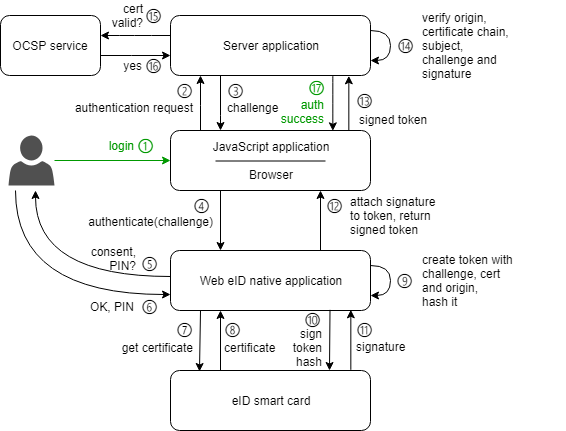
\includegraphics[scale=0.58]{webeid/Web-eID-authentication-communication-diagram}
    \caption{Web eID Authentication flow \cite{ria-webeid-systemarchitecture}}
    \label{fig:web-eid-authentication}
\end{figure}


% \subsubsection{Security Analysis}

% Arnis Paršovs

% \subsubsection{Legal Power}

% \subsubsection{Risks Transferred and other benefits}

% \subsubsection{Maturity and life use cases}

\subsubsection{Implementation}

For each protocol implementation step, developers will have to fulfill certain guarantees before the system goes into production.

\paragraph{Steps 1-3}

Building the challenge nonce. The goal of these steps is to create the challenge the user will have to sign with their private key. There are a couple of requirements the developers have to provide:
\begin{enumerate}
    \item Generated challenge nonce must be between 32 and 96 bytes (inclusive) in length \cite{ria-webeid-source-web-eid-app-authenticate};
    \item "It must be guaranteed that the authentication token is received from the same browser to which the corresponding challenge nonce was issued" \cite{ria-webeid-source-web-eid-authtoken-validation-java-readme}. The framework creators recommend attaching it to the user session.
    \item "Cache must be used for protection against replay attacks by guaranteeing that each authentication token can be used exactly once" \cite{ria-webeid-source-web-eid-authtoken-validation-java-readme}. The developers must create temporary storage for challenge nonces or any other means to revoke already used nonces.
    \item "Cookie-based authentication must be protected against cross-site request forgery (CSRF) attacks and extra measures must be taken to secure the cookies by serving them only over HTTPS and setting the HttpOnly, Secure and SameSite attributes" \cite{ria-webeid-source-web-eid-authtoken-validation-java-readme}.
\end{enumerate}

In the implementation example, these measures were addressed:
\begin{enumerate}
    \item A 64 byte cryptographically secure randomly generated nonce is created (see listing \ref{lst:web-eid-challenge}).
    \item Challenge nonce is set in the user's session, which adversaries cannot tamper.
    \item The generated nonce is stored into local memory cache for later use.
    \item A input field is rendered on the page with a unique CSRF validation token, which prevents cross-site request forgery attacks (see listing \ref{lst:web-eid-challenge-ui}).
\end{enumerate}

\begin{lstlisting}[caption={Web eID Challenge Endpoint}, label={lst:web-eid-challenge}]
private TimeSpan ChallengeLifetime { get; } = TimeSpan.FromMinutes(5);

private readonly IMemoryCache _cache; // Injected

[HttpGet("challenge")]
public IActionResult GetChallenge()
{
    var nonce = RandomNumberGenerator.GetBytes(64);

    _cache.Set(Convert.ToBase64String(nonce), true, ChallengeLifetime);
    HttpContext.Session.Set("eid.challenge", nonce);

    return Ok(new { nonce });
}
\end{lstlisting}


\begin{lstlisting}[caption={Web eID UI excerpt}, label={lst:web-eid-challenge-ui}, language={html}]
@inject Microsoft.AspNetCore.Antiforgery.IAntiforgery _csrf
@{ var csrfToken = _csrf.GetAndStoreTokens(HttpContext); }

<!-- Button used to sign in -->
<a role="button" class="btn btn-secondary" id="webeid-auth-button">Web eID</a>

<input id="csrfToken" type="hidden" value="@csrfToken.RequestToken"/>

<script>
    ...

    const authTokenResponse = await fetch("/signin-id/login", {
        method: "POST",
        headers: {
            "Content-Type": "application/json",
            "RequestVerificationToken": document.getElementById("csrfToken").value
        },
        body: JSON.stringify(...)
    });

    ...
</script>
\end{lstlisting}

\paragraph{Steps 13-17}

After the user signs the nonce challenge and sends their certificate, the server must verify its authenticity. There are a couple of steps developers must take before allowing the user to sign in.

\begin{enumerate}
    \item Verify the CSRF token from earlier steps \cite{ria-webeid-source-web-eid-authtoken-validation-java-readme}.
    \item Verify the challenge nonce came from the original user and has not expired, was not consumed.
    \item Verify the certificate validity and check if nonce was signed by the associated private key (see below).
    \item Issue an authentication token with the fields from the certificate's subject.
\end{enumerate}

In the implementation example, these measures were addressed:
\begin{enumerate}
    \item The back end endpoint for login is decorated with ValidateAntiForgeryToken Attribute. This attribute instructs the ASP.NET API to ignore requests not containing a CSRF token \cite{msdocs-anti-request-forgery}. A JavaScript application can then access the protected endpoints by providing RequestVerificationToken header (see listing \ref{lst:web-eid-challenge-ui}).
    \item The application tries to extract the challenge nonce from the browsing session. The process would succeed if the session cookie were not modified. After the extraction, the application checks the nonce cache to verify if the challenge is still active. Cache hit means the nonce has not expired, and a previous request has not consumed it already. Remove the challenge nonce from all stores.
    \item The API calls a standalone validation service to verify the nonce and certificate (see below).
    \item Application populates the ASP.NET identity management system with the fields from the certificate: serial number, given name, surname, country. An identity session cookie is sent to the client.
\end{enumerate}

\begin{lstlisting}[caption={Web eID Login Endpoint}, label={lst:web-eid-login}]
[HttpPost("login")]
[ValidateAntiForgeryToken]
public async Task<IActionResult> Login([FromBody] WebIdAuthTokenResponse token)
{
    // Obtain the challenge from session
    if (!HttpContext.Session.TryGetValue(ChallengeNonceKey, out var nonce) && nonce == null)
        return Unauthorized();

    // Check if token was not used before or expired
    var challenge = Convert.ToBase64String(nonce);
    if (!_cache.TryGetValue(challenge, out _))
        return Unauthorized();

    _cache.Remove(challenge);
    HttpContext.Session.Remove(ChallengeNonceKey);

    // Validate the certificate and signed challenge
    var validationResult = await _webEidValidationService.GetResult(new WebEidValidationRequest(token, nonce));
    if (!validationResult.Success)
        return Forbid();

    // Certificate is valid. Sign in the user

    await HttpContext.SignInAsync(BuildUser(new X509Certificate2(Convert.FromBase64String(token.UnverifiedCertificate)).Subject));

    return Ok();
}
\end{lstlisting}

\paragraph{Certificate and nonce verification}

This step is the most complicated in the entire validation process. To prevent any issues with incorrect implementation, the framework maintainers recommend using their library for validation \cite{ria-webeid-source-web-eid-authtoken-validation-java-readme}. Libraries can come with security vulnerabilities, and developers rarely update the used version; however, it is still more favorable to creating vulnerabilities from misconfiguration \cite{9240619}.

The eu.webeid.security Java package performs most of the certificate validation (expiry, purpose, policy, OCSP nonce) \cite{ria-webeid-source-web-eid-authtoken-validation-java-readme}. Still, the developer will have to configure revocation and host validation. Configuration is handled by providing a set of trusted CA certificates for trust chain verification and the hostname for challenge nonces.

\todo{This library does favor EE cards a lot more, even having hardcoded some Mobile ID policies. Not sure if it is worth mentioning.}

Because the library performs most of the heavy lifting, the developer can easily configure the validation service (see listing \ref{lst:web-eid-java-lib}).

\begin{lstlisting}[caption={Web eID Login Endpoint}, label={lst:web-eid-java-lib}]
public class AuthTokenValidatorService {

  @Bean
  public AuthTokenValidator validator() {
    try {
      return new AuthTokenValidatorBuilder()
        .withSiteOrigin(URI.create(System.getenv("ORIGIN_URL")))
        .withTrustedCertificateAuthorities(loadTrustedCACertificatesFromCerFiles())
        .build();
    } catch (JceException e) {
      throw new RuntimeException("Error building the Web eID auth token validator.", e);
    }
  }

  private X509Certificate[] loadTrustedCACertificatesFromCerFiles() {
    List<X509Certificate> caCertificates = new ArrayList<>();

    try {
      CertificateFactory certFactory = CertificateFactory.getInstance("X.509");

      File[] files = new File("/certs").listFiles((f, n) -> n.endsWith(".cer"));
      if (files != null) {
        for (File file : files) {
          try (InputStream stream = new FileInputStream(file)) {
            X509Certificate caCertificate = (X509Certificate) certFactory.generateCertificate(stream);
            caCertificates.add(caCertificate);
          }
        }
      }
    } catch (CertificateException | IOException e) {
      throw new RuntimeException("Error initializing trusted CA certificates.", e);
    }

    return caCertificates.toArray(new X509Certificate[0]);
  }
}
\end{lstlisting}

From the listing \ref{lst:web-eid-java-lib} we see that the developer needs to provide the origin URL in the form of an environment variable and to populate the folder {/certs} with trusted CA certificates.

Developers can obtain the origin URL by checking the {window.origin} of the page containing the sign-in button.

For the CA certificate set, the developers or maintainers can get an up-to-date list of trusted certificates at the EU Trust Services Dashboard \cite{eu-trustservices}. The issue with this list is that it contains all trust certificates for various scopes. In our case, we should limit the search to the extent of QCert for ESig. In the case of Estonia and Lithuania, only three entities are certified to issue certificates for QSCD (see figure \ref{fig:eu-tsp-list}). It is in stark contrast to Spain's 31 \cite{eu-trustservices}. It is possible to further narrow down to only certificate generation services for qualified certificates (CA/QC).

\begin{figure}
    \centering
    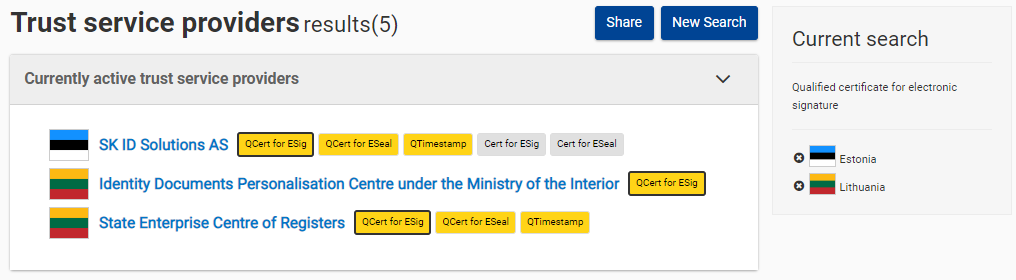
\includegraphics[scale=0.54]{webeid/eu-tsp-search}
    \caption{List of EU Trust service providers of Estonia and Lithuania capable of creating qualified certificates for e-signatures}
    \label{fig:eu-tsp-list}
\end{figure}

In the case of Estonia's single TSP, we can see that only 3 CA are currently operational (see figure \ref{fig:eu-tsp-skid}). Unfortunately, there is no standardized way of narrowing down which certificates could be used for authentication any further.

\begin{figure}
    \centering
    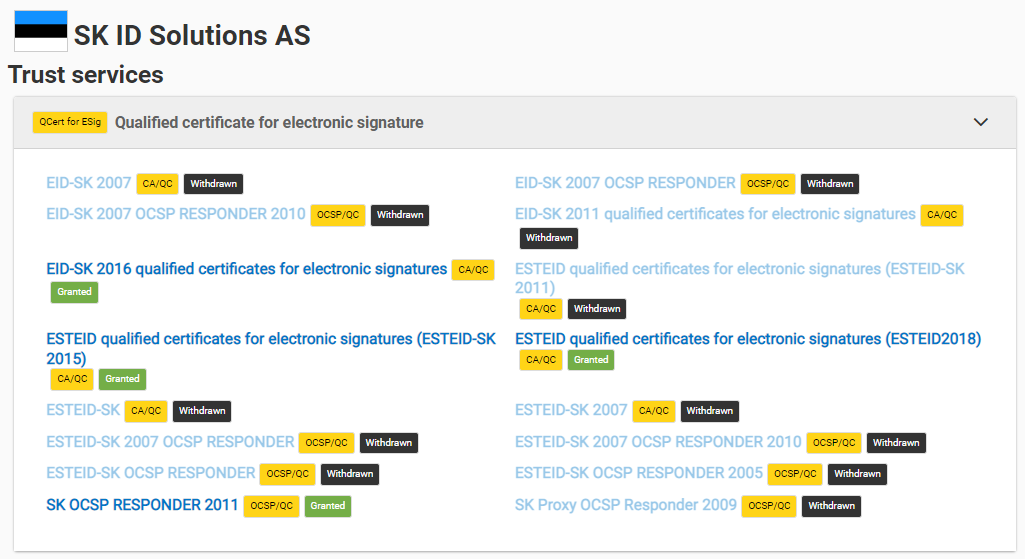
\includegraphics[scale=0.54]{webeid/eu-tsp-skid}
    \caption{List of certificates issued to SK ID Solutions AS for the purposes of Qualified certificate for electronic signature}
    \label{fig:eu-tsp-skid}
\end{figure}

An alternative way to obtain certificates 

\TODO{High-level overview of the system}
\TODO{Points of compromise?}